% !TeX root = ../document.tex
\documentclass[../document.tex]{subfiles}
\lstset{inputpath=sections}
\begin{document}

	\subsection{Simple linear regression}

	\paragraph{General}
	The output variable Y is a linear function of the input variable(s) X, where the coefficients are unknown.
	\begin{equation}
		Y \approx \beta_{0} + \beta_{1}X
	\end{equation}

	\paragraph{Estimating the coefficients}
	We need to learn the coefficients from the n training data
	\begin{equation}
	(x_{1},y_{1}),(x_{2},y_{2}),...,(x_{n},y_{n})
	\end{equation}
	And then we try to estimate the coefficients
	\begin{equation}
	\hat{y}_{i} = \hat{\beta}_{0} + \hat{\beta}_{1}x_{i}
	\end{equation}
	To test our estimated function, we define a closeness function
	\begin{equation}
		e_{i}=y_{i}-\hat{y}_{i}
	\end{equation}
	\begin{equation}
	\begin{split}
		RSS &= e^2_{1}+e^2_{2}+...+e^2_{n}\\
			&= (y_{1}-\hat{\beta}_{0} + \hat{\beta}_{1}x_{1})^2+
			(y_{2}-\hat{\beta}_{0} + \hat{\beta}_{1}x_{2})^2+...+
			(y_{n}-\hat{\beta}_{0} + \hat{\beta}_{1}x_{n})^2
	\end{split}
	\end{equation}
	To calculate the best \(\hat{\beta}_{0}\) and\(\hat{\beta}_{1}\) we can use these functions for the linear regression.
	\begin{equation}
	\begin{split}
		\overline{y}\equiv\frac{1}{n}\sum_{i=1}^{n}y_{i}\\
		\overline{x}\equiv\frac{1}{n}\sum_{i=1}^{n}x_{i}
	\end{split}
	\end{equation}
	\begin{equation}
	\begin{split}
		&\hat{\beta}_{1}=\frac{\sum_{i=1}^{n}(x_{i}-\overline{x})(y_{i}-\overline{y})}{\sum_{i=1}^{n}(x_{i}-\overline{x})^2}\\
		&\hat{\beta}_{0}=\overline{y}-\hat{\beta}_{1}\overline{x}
	\end{split}
	\end{equation}

	\paragraph{Accuracy of the coefficient estimates}
	We assume this true relationship, where the function f is unknown and the error is random with zero mean.
	\begin{equation}
	\begin{split}
		Y &= f(X) + \epsilon\\
		Y &= \beta_{0} + \beta_{1}X+\epsilon
	\end{split}
	\end{equation}
	Now the error term is a catch-all for everything that is missed by the simple linear model. We usually assume that the error term is independent of the data X. This model is called the population regression line, which is the best (in minimum RSS sense) linear approximation.\\
	But we can't estimate the function correctly and have to use the mean-error, that's exactly the same problem with the coefficients, which have also a mean-error, which depends on the bias.
	The function for \(\overline{y}\) and \(\overline{x}\) is unbiased and on average correct. That means, that the sum over these parameters as used in \(\hat{\beta}_{1}\) and \(\hat{\beta}_{0}\) is also on average correct.
	\begin{center}
		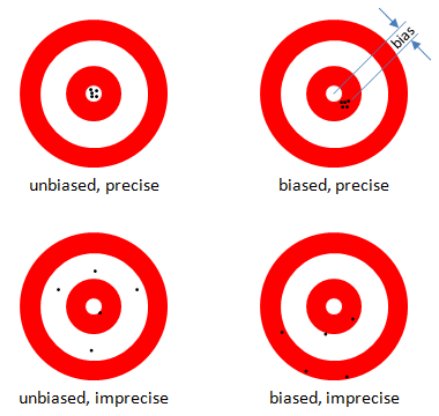
\includegraphics[width=.6\textwidth]{pictures/bias_precision.png}
	\end{center}
	\subparagraph{true variance}
	But this unbiased approach is not enough to be accurate as shown above.
	We also require a small variance of the estimate or equivalently a small standard error. This is the variance for the function Y.
	\begin{equation}
		Var(\hat{\mu})=SE(\hat{\mu})^2=\frac{\sigma^2}{n}
	\end{equation}
	The variance of Y is inversely proportional to the number of observations (more observation, less error)
	\begin{equation}
	\begin{split}
		SE(\hat{\beta}_{0})^2&=\sigma^2(\frac{1}{n}+\frac{\overline{x}^2}{\sum_{i=1}^{n}(x_{i}-\overline{x})^2})\\
		SE(\hat{\beta}_{1})^2&=\frac{\sigma^2}{\sum_{i=1}^{n}(x_{i}-\overline{x})^2}
	\end{split}
	\end{equation}
	In these formulas we assume that the errors for each observation are uncorrelated with the common variance. The standard error for the slope \(\hat{\beta}_{1}\) is smaller when the X data is more spread out. Further note that the standard error for the intercept \(\hat{\beta}_{0}\) would be the same as for the sample mean of y, if the sample mean of x would be zero.\\
	Unfortunately, the required variance is not known, but we can estimate it from the data
	\begin{equation}
		\sigma^2 = Var(\epsilon)
	\end{equation}
	\subparagraph{estimated variance}
	When we want to estimate the variance from the data, we use the residual standard error
	\begin{equation}
		RSE = \sqrt{\frac{RSS}{(n-2)}}
	\end{equation}
	And now the confidence intervals can be calculated using the standard errors. We usually want the 95\% confidence interval
	\begin{equation}
	\begin{split}
		\hat{\beta}_{1}\pm 2*SE(\hat{\beta}_{1})\\
		\hat{\beta}_{0}\pm 2*SE(\hat{\beta}_{0})
	\end{split}
	\end{equation}
	\subparagraph{hypothesis}
	Now hypothesis tests on the coefficients (parameters) can be calculated using the standard errors. We test the null hypothesis versus the alternative hypothesis. If there is no relationship, we would expect the slope to be zero.
	\begin{equation}
	\begin{split}
		&H_{0}: \text{There is no relationship between X and Y}\\
		&H_{0}: \beta_{1}=0\\
		&H_{a}: \text{There is some relationship between X and Y}\\
		&H_{a}: \beta_{1} \ne 0
	\end{split}
	\end{equation}
	Since the slope is never really exactly zero, we need to measure how far away the slope is from zero. Hence the solution is to express the estimate of the slope in multiples of the standard error, calculating the so called t-statistic.
	\begin{equation}
		t = \frac{\hat{\beta}_{1}-0}{SE(\hat{\beta}_{1})}
	\end{equation}
	Since the t-distribution is a family of distributions, it is important to know which one to use and this depends on the number of training samples.
	For example, if n=30 then the p-value thresholds for rejecting the null-hypothesis is 1\%(5\%) imply that a t-statistic of around 2.75(2) is enough to reject the null-hypothesis.\\
	Hence for p=1\%, if the estimate of the slope is about 2.75 times the standard error removed from 0, then we conclude that there is a relationship between X and Y.

	\paragraph{Accuracy of the model}
	The quality of a linear regression fit is usually assessed using the residual standard error and the \(R^2\) statistic.
	\begin{equation}
		Y = \beta_{0} + \beta_{1}X + \epsilon
	\end{equation}
	\begin{equation}
		RSS = \sum_{i=1}^{n}(y_{i}-\hat{y}_{i})^2
	\end{equation}
	\begin{equation}
		RSE = \sqrt{\frac{RSS}{n-2}} = \sqrt{\frac{\sum_{i=1}^{n}(y_{i}-\hat{y}_{i})^2}{n-2}}
	\end{equation}
	The RSE provides an absolute measure of lack of fit of the model to the data. RSE carries the same unit as Y. The \(R^2\) statistic provides an alternative measure of fit, which takes the form of a proportion between 0 and 1.
	\begin{equation}
		TSS = \sum(y_{i}-\overline{y})^2
	\end{equation}
	\begin{equation}
		R^2 = \frac{TSS - RSS}{TSS} = 1-\frac{RSS}{TSS}
	\end{equation}
	The \(R^2\) measures the proportion of variability in Y that can be explained using X. A \(R^2\) value close to one means that a large part of the variability in the response has been explained by the regression, a value close to zero means that most of the variability in the response could not be explained by the regression. This could be because the relationship is highly non-linear and/or the inherent random error is already high. Nevertheless, it is not clear what a "good" \(R^2\) statistic should be.\\
	For simple linear regression the \(R^2\) statistic is identical to the sample correlation squared.
	\begin{equation}
		Cor(X,Y)=\frac{\sum_{i=1}^{n}(x_{i}-\overline{x})(y_{i}-\overline{y})}{\sqrt{\sum_{i=1}^{n}(x_{i}-\overline{x})^2}\sqrt{\sum_{i=1}^{n}(y_{i}-\overline{y})^2}}
	\end{equation}

	\subsection{Multiple linear regression}

	\paragraph{Estimating the coefficients}
	Instead of doing each media (in the example) separately, a joint approach is more promising, since the correlations between the media can be captured.
	\begin{equation}
		Y = \beta_{0}+\beta_{1}X_{1}++\beta_{2}X_{2}+...+\beta_{n}X_{n}+\epsilon
	\end{equation}
	Just as in the simple regression case, the coefficients (parameters) are estimated in such a way, that the sum of squared residuals in the training data is minimized.
	\begin{equation}
	\begin{split}
		RSS &= \sum_{i=1}^{n}(y_{i}-\hat{y}_{i})^2\\
			&= \sum_{i=1}^{n}(y_{i}-\hat{\beta}_{0}-\hat{\beta}_{1}x_{i1}-\hat{\beta}_{2}x_{i2}-...-\hat{\beta}_{n}x_{in})^2
	\end{split}
	\end{equation}

	\paragraph{Is there a relationship between response and predictors}
	To define if the predictors have an influence on the response we have a hypothesis.
	\begin{equation}
	\begin{split}
		&H_{0}:\beta_{1}=\beta_{2}=...=\beta_{p}=0\\
		&H_{a}:\text{At least one }\beta_{j}\text{ is non-zero}\\
	\end{split}
	\end{equation}
	The statistic used to make a decision if the hypothesis is significant or not, is called F-statistic.
	\begin{equation}
		F = \frac{\frac{TSS-RSS}{p}}{\frac{RSS}{n-p-1}}
	\end{equation}
	\(p\) is the number of predictors and \(n\) is the number of training samples.
	Given n and p, the F-distribution is completely defined and therefore the p-value can be calculated. And this p-value can be used to decide if the null hypothesis should be accepted or rejected.\\
	So far we tested if all coefficients are zero. Sometimes one wants to test if a certain subset of q coefficients are zero.
	\begin{equation}
		H_{0}: \beta_{p-q+1}=\beta_{p-q+2}=...=\beta_{p}=0
	\end{equation}
	Now we fit a second model that uses all the predictor variables except the last q and the result in a residual sum of squares called \(RSS_{0}\)
	\begin{equation}
		F = \frac{\frac{RSS_{0}-RSS}{q}}{\frac{RSS}{n-p-1}}
	\end{equation}
	Assume we only leave out one predictor variable, then the appropriate F-statistic (and the associated p-value) would tell us the partial effect of adding that left out variable to the model. It turns out, the F-statistic, if only one variable is left out, is identical to the squared t-statistic.

	\paragraph{Deciding on important variables}
	Once the overall F-statistic p-value has been calculated and it is smaller than 1\% (5\%), then at least one predictor is significantly associated with response. So to find out, which predictors are actually associated, we could do an exhaustive search, but this is really slow. Other approaches are called forward selection, backward selection and mixed selection, where all approaches are greedy ones.

	\paragraph{Model fit}
	As in the simple linear regression the two most common measures are the RSE (residual standard error) and \(R^2\)
	\begin{equation}
	\begin{split}
		&RSE = \sqrt{\frac{RSS}{n-p-1}}\\
		&R^2 = \frac{TSS-RSS}{TSS}=1-\frac{RSS}{TSS}
	\end{split}
	\end{equation}
	In simple linear regression \(R^2\) is equal to the square of the correlation coefficient between the response and the predictor variable.\\
	In multiple linear regression it turns out that \(R^2\) is equal to the squared correlation coefficient between the true response and the response predicted by the linear model.
	\begin{equation}
		R^2=Cor(Y,\hat{Y})^2
	\end{equation}
	A value close to 1 indicates that the model explains a large portion of the variance in the response variable.

	\paragraph{Prediction}
	Once the multiple linear regression model has been trained, it is simple to use it for prediction. There are three types of uncertainties associated with this prediction.
	\begin{description}
		\item The coefficients \(\hat{\beta}_{0},\hat{\beta}_{1},...\) are estimates for the real \(\beta_{0},\beta_{1},...\) and its only an estimate for a plane. The inaccuracy in the coefficient estimates is related to the reducible error. We can compute the confidence interval in order to determine how close \(\hat{Y}\) will be to \(f(X)\)
		\item Of course, in practice assuming a linear model is almost always an approximation of reality, so there is an additional source of potentially reducible error which we call model bias. However, here we will ignore this discrepancy, and operate as if the linear model were correct.
		\item Even if we knew the true values for the coefficients, the response value cannot be predicted perfectly because of the random error, which we referred as the irreducible error. We use prediction intervals to answer how much will \(Y\) vary from \(\hat{Y}\). These intervals are always wider than confidence intervals, because they incorporate both the error in the estimate (reducible error) and the uncertainty as to how much an individual point will differ from the population regression plane (irreducible error)
	\end{description}

	\subsection{Other consideration in the regression model}

	\paragraph{Qualitative predictors}
	So far all predictors had numerical values, so called quantitative predictors. In many cases, some predictor variables are of qualitative nature. Qualitative predictors are predictors with only two levels and we need an indicator or dummy variable, which can take on two different numerical values, usually 0 or 1.
	\begin{equation}
	\begin{split}
		&x_{i}=\begin{cases}
			1 &\text{if ith person is female}\\
			0 &\text{if ith person is male}
		\end{cases}\\
		&y_{i} = \beta_{0}+\beta_{1}x_{i}+\epsilon_{i}=\begin{cases}
			\beta_{0}+\beta_{1}+\epsilon_{i} &\text{if ith person is female}\\
			\beta_{0}+\epsilon_{i} &\text{if ith person is male}
		\end{cases}
	\end{split}
	\end{equation}
	The decision which number (1 or 0) is male/female is arbitrary. If we would have chosen to represent male with a 1 and female with a 0, the regression would have given the same result, but the interpretation would have to be consistent with the definition.\\
	Another scheme to code such two level predictor variables does not use the 0/1 scheme but a -1/+1 scheme
	\begin{equation}
	\begin{split}
	&x_{i}=\begin{cases}
	1 &\text{if ith person is female}\\
	-1 &\text{if ith person is male}
	\end{cases}\\
	&y_{i} = \beta_{0}+\beta_{1}x_{i}+\epsilon_{i}=\begin{cases}
	\beta_{0}+\beta_{1}+\epsilon_{i} &\text{if ith person is female}\\
	\beta_{0}-\beta_{1}+\epsilon_{i} &\text{if ith person is male}
	\end{cases}
	\end{split}
	\end{equation}
	When we have qualitative predictors with more than two levels, we need more than one dummy variable. We need at least as many dummies as levels-1.
	\begin{equation}
	\begin{split}
	&x_{i1}=\begin{cases}
	1 &\text{if ith person is Asian}\\
	0 &\text{if ith person is not Asian}
	\end{cases}\\
	&x_{i2}=\begin{cases}
	1 &\text{if ith person is Caucasian}\\
	0 &\text{if ith person is not Caucasian}
	\end{cases}\\
	&y_{i} = \beta_{0}+\beta_{1}x_{i1}+\beta_{2}x_{i2}\epsilon_{i}=\begin{cases}
	\beta_{0}+\beta_{1}+\epsilon_{i} &\text{if ith person is Asian}\\
	\beta_{0}+\beta_{2}+\epsilon_{i} &\text{if ith person is Caucasian}\\
	\beta_{0}+\epsilon_{i} &\text{if ith person is African America}\\
	\end{cases}
	\end{split}
	\end{equation}
	The level without dedicated dummy variable is called the baseline. Clearly the coefficients and the associated p-values do depend on the selected coding of the dummy variable. Hence instead of relying on the individual coefficients and their p-values, we better focus on the F-test which does not depend on the particular coding.

	\paragraph{Removing additivity assumption}
	The linear model assumes that the relationship between the predictors and the response are additive and linear. Hence we remove the additivity assumption. \\
	Consider the standard linear regression model with two predictors.
	\begin{equation}
	\begin{split}
		Y &= \beta_{0}+\beta_{1}X_{1}+\beta_{2}X_{2}+\epsilon\\
		&=\beta_{0}+\beta_{1}X_{1}+\beta_{2}X_{2}+\beta_{3}X_{1}X_{2}+\epsilon\\
		&=\beta_{0}+(\beta_{1}+\beta_{3}X_{2})X_{1}+\beta_{2}X_{2}+\epsilon\\
		&=\beta_{0}+\tilde{\beta}_{1}X_{1}+\beta_{2}X_{2}+\epsilon\\
		\tilde{\beta}_{1}&=\beta_{1}+\beta_{3}X_{2}
	\end{split}
	\end{equation}
	We added a cross term to the equation so that the slope of \(X_{1}\) now clearly depends on \(X_{2}\) so adjusting \(X_{2}\) will change the impact of \(X_{1}\) on Y\\
	There can also be interaction terms between qualitative variables as well as between qualitative and quantitative variables.
	\begin{equation}
	\begin{split}
		Y &\approx \beta_{0}+\beta{1}X_{1}+\begin{cases}
			\beta_{2}+\beta_{3}X_{1} &\text{if student}\\
			0 &\text{if not student}
		\end{cases}\\
		&=\begin{cases}
			(\beta_{0}+\beta_{2})+(\beta_{1}+\beta_{3})X_{1} &\text{if student}\\
			\beta_{0}+\beta_{1}X_{1} &\text{if not student}
		\end{cases}
	\end{split}
	\end{equation}

	\paragraph{Non-linear relationships}
	The simplest extension of the linear models to non-linear problems is called polynomial regression. The simplest approach to allow for a non-linear relationship is to add transformed versions of the predictors to the model.
	\begin{equation}
		Y = \beta_{0}+\beta_{1}x+\beta_{2}x^2+\epsilon
	\end{equation}
	But we have to be careful to not overtrain the model with higher orders.

	\paragraph{Potential problems}
	While linear models are powerful there are a list of potential problems, one needs to be aware of
	\subparagraph{Non-linearity of data}
	The linear regression models assumes that there is a straight line relationship between the predictors and the response. This is almost never the case and hence we need to be able to judge how well the linear model is approximating the real world.\\
	Plotting the residuals as a function of the predicted response help identifying linearity problems. The residuals should be randomly scattered around zero ant there should be no visible pattern.\\
	If the residual plot indicates that there are non-linear associations in the data, then a simple approach is to use non-linear transformations of the predictors, such as \(log(x), \sqrt{x}\) and \(x^2\), in the regression model.
	\subparagraph{Correlation of error terms}
	An important assumption is, that the error terms are uncorrelated and this is called noise. If the error terms are correlated, then the standard error terms are too small and this leads to confidence and prediction intervals that are to narrow. This leads to p-values that are too low.\\
	In general the assumption that the errors are uncorrelated is very important for linear regression and other statistical methods and hence care should be taken when designing experiments to measure data, such that such correlations are not introduced.
	\subparagraph{Non-constant variance of error}
	We assume that the error terms have a constant variance, the standard errors, confidence intervals and hypothesis test depend on this. But unfortunately, this assumption is sometimes violated.\\
	Often the error term is correlated with the response. Higher responses have higher errors. Or in other words, the errors are proportional to the response.\\
	Identifying non-constant variances in the errors uses the residual plot, where the envelope of the residuals is not constant, but for example, a funnel.\\
	One solution to the funnel problem is to transform the response using an inverse function such as log(Y) or sqrt(Y). This will shrink the larger responses and hence reduce the effect.
	\subparagraph{Outliers}
	An outlier is a point for which the true response is far away form the predicted response and it belongs to common predictor values.\\
	In this case, excluding the outlier does not really change the least squares fit, but it does change the performance measures.\\
	The residual plot can be used to identify outliers and then we can calculate the studentized residuals.
	\begin{equation}
	\frac{\hat{\epsilon}_{i}}{\sigma\sqrt{1-h_{i}}}
	\end{equation}
	A value over 3 defines an outlier.
	\subparagraph{High leverage points}
	A high leverage point is a data point with an unusual predictor value. In this case, removing the data point changes the least squares fit significantly. Such problematic high leverage points need to be identified and removed. \\
	\begin{equation}
		h_{i} = \frac{1}{n}+\frac{(x_{i}-\overline{x})^2}{\sum_{i'=1}^{n}(x_{i'}-\overline{x})^2}
	\end{equation}
	In order to quantify an observation's leverage, the leverage statistic can be computed as shown above for simple linear regression, which takes on values between 1/n and 1. The average leverage for all observations has a leverage greatly exceeding (p+1)/n, then we can assume that that point is a high leverage point.
	\subparagraph{Collinearity}
	Two or more predictors are highly correlated, hence it is not clear how to distribute the slope to the two or more predictors. \\
	This reduces the accuracy of the estimation of the slopes. Hence the standard errors grow which in turn results in smaller t-statistics which in turn results in larger p-values.\\
	I there is a collinearity between only two predictor variables, then simply inspecting the (normalized) correlation matrix will show a high correlation between them, if there is a collinearity between more than two variables, a more sophisticated approach needs to be used called the variance inflation factor VIF.
	\begin{equation}
		VIF(\hat{\beta}_{j})=\frac{1}{1-R^2_{X_{j}|X_{-j}}}
	\end{equation}
	The minimum of VIF is 1, which indicates a complete lack of collinearity. As a rule of thumb, values above 5 to 10 indicate a problem with collinearity.\\
	Once the variables with collinearity are detected, there are two obvious solutions:
	\begin{itemize}
		\item Drop one of the problematic variables
		\item Combining collinear predictor variables into a new variable
	\end{itemize}

	\subsection{Comparison of linear regression with KNN}
	Linear regression is a parametric approach. If the linearity assumption holds, this will result in good results which are easy to interpret. If the assumption does not hold, this will result in a low performing scheme.\\
	The KNN regression is a non-parametric approach and hence there are no assumptions that can be violated. But the results are often hard to interpret and it usually takes much more training data to achieve similar performance. The KNN regression is very similar to KNN classification but the main difference is, that there is no voting among the K nearest neighbors in the set \(N_{0}\) for the winning class, but an average is performed for the prediction value.
	\begin{equation}
		\hat{f}(x_{0})=\frac{1}{K}\sum_{x_{i}N_{0}}y_{i}
	\end{equation}
	When K=1 results in a very rough approximation which has a large variance, since every training point is directly used in the solution. Hence larger variance, but lower bias.\\
	When K=9 results in a smoother approximation. Here the variance is clearly smaller, since every training point is averaged with eight others, but the bias increases. Hence lower variance, but higher bias.\\
	A parametric approach will outperform an non-parametric approach, when the assumed parametric form is close to the true form of f() or if there is not much training data. If the true f is linear, linear regression should be unbeatable. If it's a small non-linearity, the simple linear regression approach and the KNN regression scheme are similar, but if the non-linearity becomes stronger, the KNN regression scheme outperforms the simple linear regression approach.\\
	When we have many predictor variables, this becomes a high dimensional problem, where we never have enough training data for parametric approaches.
\end{document}
